%!TEX root = ../../main.tex
\chapter{ユーザースキルの推薦機構}
本章ではユーザースキル推薦機構について述べる

\section{スキルタグ}
ユーザーはタスクに対して,そのタスクの完了に必要なスキルタグを登録することができる.

\section{ユーザースキル}
ミッション内の完了したタスクについて,完了したユーザーがそのタスクに紐付いているスキルタグのスキルを有しているということになる.
このスキルタグを単純に出現回数順に推薦するのではなく,そのタスクの前後関係や,ミッション内での位置を考慮して重み付けを行う.
以下にそのアルゴリズムを述べる.


\ref{img:large_mission}

\begin{figure}[t]
	\begin{center}
		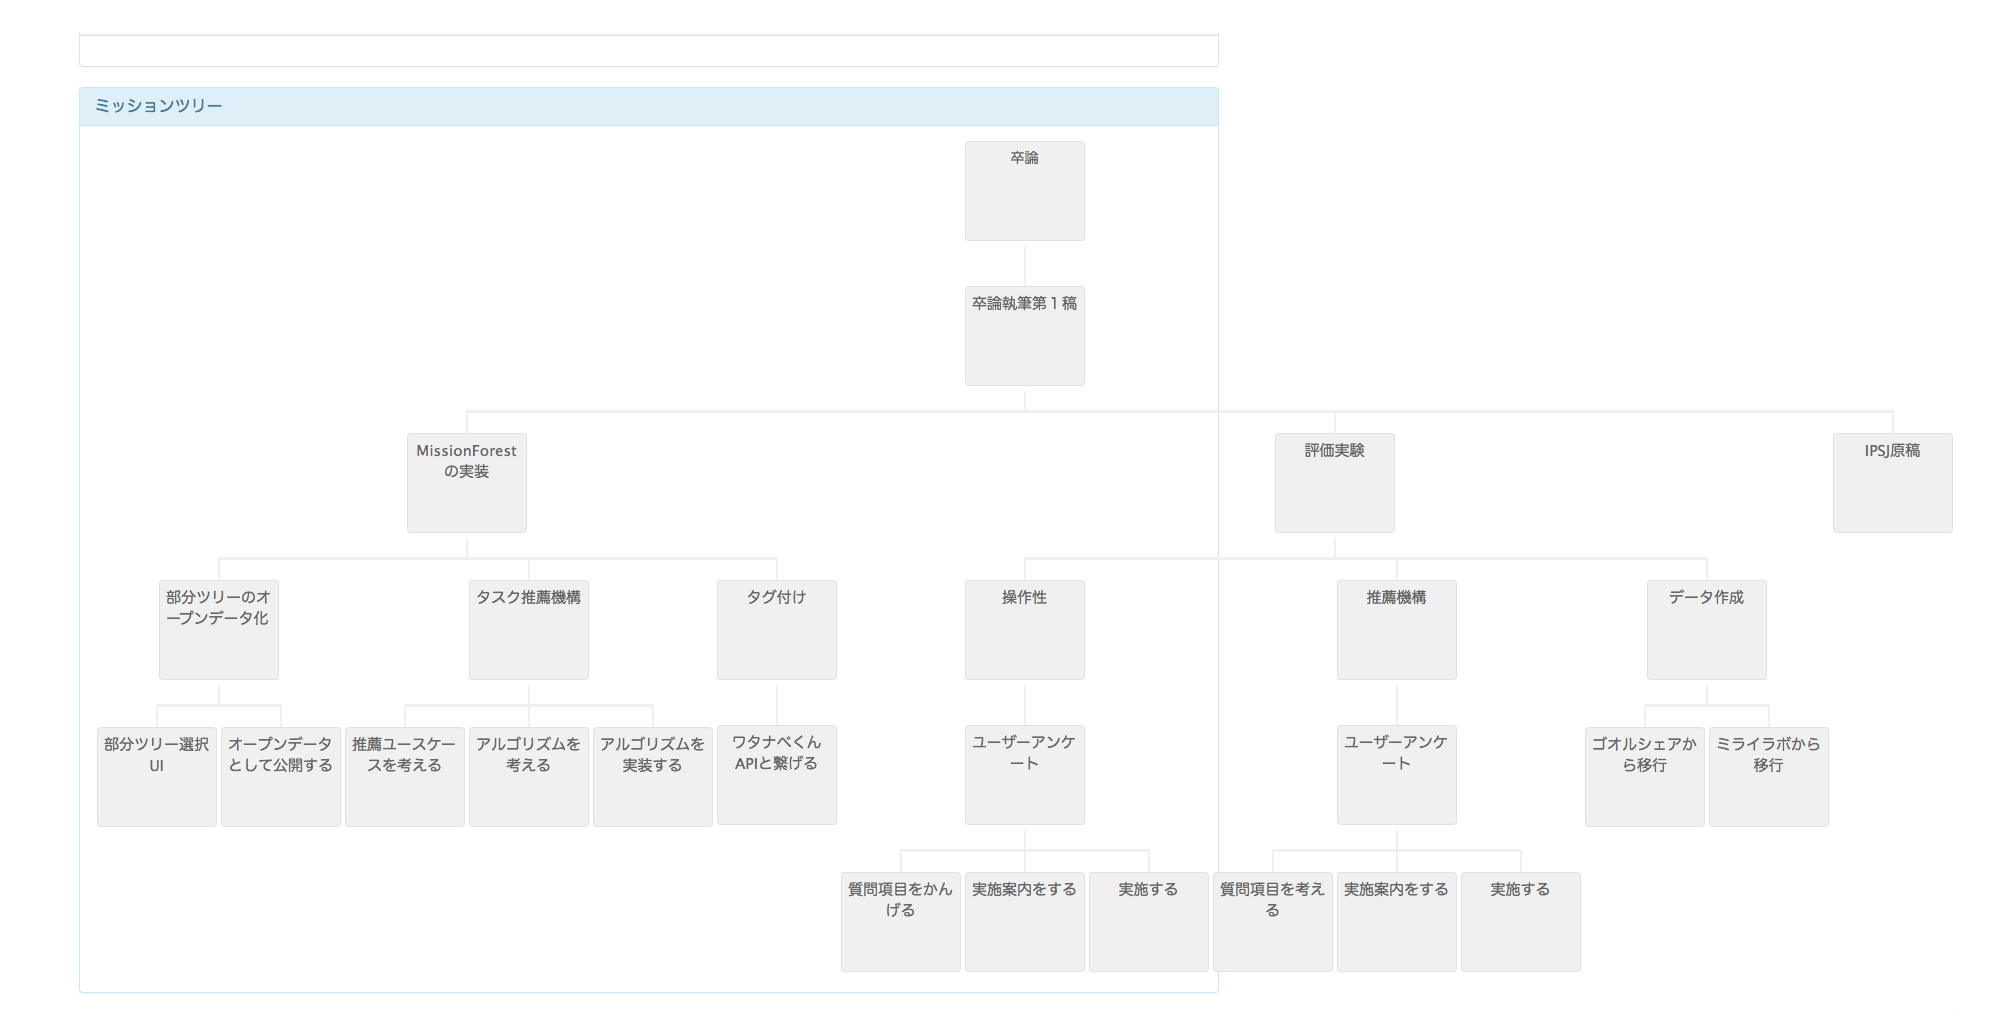
\includegraphics[width=0.9\linewidth]{assets/img/large_mission.png}
		\caption{ゴオルシェア実験結果}
		\label{img:large_mission}
	\end{center}
\end{figure}

\section{推薦手法の考察}

\subsection{出現回数を用いる}

\subsection{タスクの階層を用いる}

\subparagraph{タスク完了までの時間を用いる}
